\documentclass[12pt]{article}

\usepackage{sbc-template}

\usepackage{graphicx,url}

\usepackage[brazil]{babel}   
%\usepackage[latin1]{inputenc}  
\usepackage[utf8]{inputenc}  
% UTF-8 encoding is recommended by ShareLaTex
\usepackage{graphicx}
     
\sloppy

\title{Jogo - Avaliação de Transtorno de Ansiedade}

\author{Ariel R. Nessi, Cristian Cotrena, Matheus S. Redecker}


\address{Pontifícia Universidade Católica do Rio Grande do Sul - PUCRS}


\begin{document} 

\maketitle

\begin{abstract}
This article has as objective to describe the system named Pequira and its features. Your modalagem of IHC will be shown, along with their scenarios and goals.
\end{abstract}
     
\begin{resumo} 
  Este artigo tem como o objetivo descrever o sistema Pequira e suas funcionalidades. A sua modelagem de IHC será mostrada, junto com seus cenários e metas.
\end{resumo}


\section{Introdução}


\paragraph{} O sistema Pequira tem o objetivo de ajudar os pacientes com transtornos de ansiedade possibilitando um acompanhamento em casa ou no próprio consultório com tarefas propostas pelo médico. O médico consegue atribuir tarefas que devem ser realizadas, com as quais é feito o monitoramento das ondas cerebrais do paciente e com isso fornecer subsídios para o tratamento da próxima consulta ou ainda auxiliar o paciente em superar seu transtorno através de atividades que testem a reação do paciente  em situações de estresse.
\paragraph{} Em relação a usabilidade, alguns cuidados são observados, como a pausa de uma atividade no caso do abandono do paciente, detectada através da webcam, nesta situação a atividade é pausada e o retorno só é permitido através de uma nova autenticação por reconhecimento facial.

%temos os tratamentos de erros em relação ao usuário sair de frente da aplicação no meio de uma tarefa, se isso acontecer a tarefa terá uma pausa e um timer vai ser disparado para que tenha o controle do tempo que ele esteve fora para que depois ele tenha que justificar para o médico porque ele não fez de forma continua a tarefa, 

O sistema não será projetado para comportar usuários com qualquer tipo de deficiencia visual ou auditiva, pois as atividades desenvolvidas fazem uso de recursos audiovisual e portanto uma adaptação para usuários especiais seria necessaria para cada atividade proposta no sistema.

%em relação a acessibilidade não teremos tratamento para pessoas com deficiência visual ou auditiva, pois o sistema possui interação audiovisual com o usuário e para isso ser adaptado teriam que ser feitas mudanças de projetos que não estão prevista para essa versão do sistema.
\paragraph{}A motivação para o desenvolvimento desse trabalho se deu ao fato de que muitas pessoas precisam de um acompanhamento mais intenso do seu quadro emocional e, as vezes, por várias questões, esse acompanhamento não é feito de forma plenamente satisfatória à fim de que o paciente tenha uma recuperação mais eficiente e definitiva. Com o Pequira disponibilizamos um melhor acompanhamento e uma melhor resposta ao diagnostico, pois, o paciente pode visualizar seu progresso durante o tratamento.

%da forma que precisaria ser feito para que o paciente tenha uma melhora mais intensa e com menos recaídas. Com o Pequira teremos um melhor acompanhamento e uma melhor resposta ao diagnostico, pois, o paciente estará vendo sua evolução e saberá os pontos que devem ser aprimorados.

\section{Sistema}

\paragraph{}O Sistema vem armazenado em um pendrive executável, este sistema possui um conjunto de testes nos quais as ondas cerebrais do usuário são captadas a fim de auxiliar no diagnóstico de determinados tipos de transtornos de ansiedade.

\paragraph{}Trabalhamos neste sistema com três patologias especificas. 
\begin{enumerate}
\item Ataque de pânico;
\item Transtorno de pânico com agorafobia;
\item Transtorno Obsessivo-Compulsivo.
\end{enumerate}

\paragraph{}Para que o sistema consiga captar as ondas cerebrais e identificar sintomas, o usuário vai utilizar um hardware chamado Emotiv que vai captar as ondas  durante a utilização do sistema e armazena-las no pendrive executável no fim dos testes.
\paragraph{}Os dispositivos de entrada e saída utilizados pelo sistema são: Pendrive executável; Emotiv; Teclado; Mouse; Webcam; Monitor. Para iniciar o sistema, o usuário deve obrigatoriamente estar com o Pendrive, Webcam, Monitor e o Emotiv conectado ao Computador, ao ligar o sistema o usuário recebe instruções de como colocar e usar o Emotiv.
\paragraph{}Todas as informações sobre o usuário são armazenadas no Pendrive executável e só podem ser consultadas mediante a uma senha, garantindo assim a segurança das informações contidas nele.
\paragraph{}Durante os jogos, o sistema vai expor o usuário a uma situação associada a seu tipo específico de Transtorno de ansiedade e, a partir disso, vai analisar seu comportamento pelo Emotiv e a Webcam assim podendo ter um acompanhamento mais preciso da patologia do paciente.

%muito melhor do grau da doença do paciente.


\section{Modelagem} \label{sec:firstpage}

\begin{enumerate}
\item Qual a finalidade do Pequira? %1 OK
\item Existe a possibilidade de se jogar online? %2 OK
\item Qual a plataforma escolhida para o sistema? %3 OK
\item Que tipos de distúrbios serão tratados? %4 OK
\item Que tipos de informações de cada sessão serão salvas? %5 OK
\item Que tipo de interação o psiquiatra consegue ter com o sistema? %6  OK
\item Como será a estrutura dos jogos? %7  OK
\item Como é feito o acompanhamento do psiquiatra com o paciente? %8  OK
\item Que tipo de liberdade o usuario tem para acessar o jogo? %9  OK
\item O que tipo de configurações o psiquiatra tem acesso? %10
\item De que modo as configurações entram em vigor?  %11 ok
\item Que tipo de informações o paciente tem acesso? %12 ok
\item Como questões de sigilo são tratadas? %13 ok
\end{enumerate}

\newpage
\subsection{Cenário 1 - Novo paciente no consultório}
Abrange as perguntas: 1,2,3,4,5

\paragraph{} Rita acaba de marcar sua primeira consulta no consultório Gaúcho Guapo que utiliza-se do sistema Pequira para diagnosticar e auxiliar no tratamento de seus pacientes [1]. Em sua primeira sessão é atendida pelo psicólogo Pedro, este acredita de que Rita sofra de distúrbios de ansiedade e então decide usar o Pequira para melhor embasar suas suspeitas [4]. Como se trata da primeira sessão, Pedro decide executar o jogo no próprio consultório, para assim poder instruir Rita a como proceder em casa em seu computador doméstico [3]. Primeiro Pedro entra com sua senha no Pequira, busca entre a lista de jogos, um apropriado para ataques de pânico [4], então, coloca Rita em frente ao computador, posiciona o equipamento Emotiv em sua cabeça e alinha uma Webcam a fim de captar o seu rosto[5], convenientemente o telefone de Pedro toca e ele encontra ali a desculpa que necessitava para deixar Rita sozinha com a máquina, ele assim inicia o jogo e deixa Rita. Pedro sabe que o jogo dura 10 minutos e não depende nem possui nenhuma capacidade de conexão com a internet [2] e então vai tomar um café enquanto espera Rita acabar sua sessão. Em precisos 10 minutos Pedro volta à sua sala e encontra Rita removendo o Emotiv, Rita questiona se é possível executar os jogos em seu tablet, mas infelizmente Pedro responde que o sistema é compatível apenas com sistemas desktops [3]. Pedro então se senta em frente à máquina e rapidamente analisa os resultados de Rita, entre as ondas de excitação instantânea, excitação de longo termo, frustração, engajamento, meditação, interesse e afinidade[5] o psicólogo está interessado nas métricas de frustração que o sistema providencia, mas nada alarmante aqui. Contudo ele nota que o sistema captou entradas no teclado, em um jogo de concentração sem interação por este dispositivo. Ao verificar nota que Rita pressionou repetidamente a tecla espaço nos momentos em que sua frustração subia [5]. 


\subsection{Cenário 2 - A volta do paciente para a casa}
Abrange as perguntas: 6,7,8,9,10

\paragraph{} 
Pedro, após a primeira consulta configura uma lista de jogos para o tratamento de Rita, bem como eventos de interesse no jogo, neste caso ele configura o sistema para colocar marcadores nos momentos que o personagem de Rita morre nas partidas [6]. Os jogos selecionados deliberadamente causam o jogador à perder uma porção de vezes à fim de causar frustração no usuário [7]. Ao entregar o pendrive à Rita, Pedro explica que os jogos no sistema farão parte do tratamento e instrui Rita que as atividades deverão ser executatas entre o horário das 21:00 e 22:00 horas, por um período de até 30 minutos, bem como fornece à Rita uma senha de acesso ao sistema [10].
No final do dia, Rita já cansada se dirige à seu computador para dar continuidade no seu tratamento. Insere o pendrive no computador e digita sua senha de acesso ao sistema, o sistema prontamente solicita à Rita que conecte à máquina o Emotiv e a webcam, após fazer os ajustes solicitados o sistema faz a calibragem dos periféricos e Rita começa sua sessão de jogos. Durante a sessão o sistema coleta as ondas produzidas por Rita nos diversos momentos do jogo e os armazena no pendrive. \\
No dia seguinte durante sua sessão Rita é interrompida por uma ligação e deixa o computador para atender o telefone, ao retornar encontra o Pequira pausado solicitando uma nova calibragem e autenticação do usuário para prosseguir no jogo [6]. Ansiosa para saber de seus resultados no dia seguinte Rita entra em contato com Pedro, para questionar como acessar as informações de sua sessão, Pedro responde que ela terá acesso na sua próxima consulta e que deve trazer seu pendrive para que possa ser analisado [8].
%Pedro, psicólogo, pós uma consulta organiza um conjunto de jogos à seu critério no Pequira com base na consulta feita [7] e, entrega a Rita um Pendrive com o sistema Pequira junto ao Emotiv explicando que o Pequira faz parte de seu tratamento permitindo que Rita utilize-o em sua residência [9], estabelecendo um período de uso de 30 minutos diários em um intervalo entre 21:00hrs à 22:00hrs [10] ,explica também a forma de uso no Desktop junto aos demais dispositivos de entrada e saída e cadastra uma senha de acesso para Rita acessar o sistema. 
%Rita agradece Pedro pela consulta e retorna para sua casa, ao fim do dia, decide usar o Pequira, não lembrando exatamente a orientação que Pedro passou sobre a forma de uso, Rita apenas pluga o Pendrive em seu Desktop e digita a senha para ter acesso ao Pequira. O sistema, identificando que, faltavam dispositivos, enviou uma mensagem de texto orientando como plugar o USB do Emotiv em seu computador e solicitou também que liga-se a Webcam, Rita concluiu os procedimentos solicitados, feito isso, o sistema orientou de como colocar e calibrar o Emotiv em sua cabeça e arrumar a posição da Webcam.
%Rita inicia os testes organizados por Pedro, durante esse uso, o sistema foi armazenando os dados no Pendrive, concluindo seu prazo de 30 min diário, Rita desliga o sistema. 
%No dia seguinte Rita foi trabalhar pela manha e João, irmão de Rita, curioso ao ver o Emotiv decide utiliza-lo, ao ligar o sistema, o Pequira bloqueia o acesso informando que ainda não esta no horário programado para o uso impedindo João de acessar os dados [10].
%Rita chega do trabalho e decide utilizar novamente o Pequira, após ter utilizado por 15 min, o telefone residencial toca e Rita retira o Emotiv e vai atende-lo, durante isso, o sistema é pausado automaticamente e manda uma mensagem na tela informando a Rita que ela ainda precisa cumprir mais 15 min para concluir a meta do dia [6], ao retornar, Rita calibra o Emotiv em sua cabeça, digita sua senha e continua seu teste. No dia seguinte, empolgada com o tratamento, Rita liga para seu psicólogo e pergunta qual procedimento deve ser feito no Pequira para ter acesso ao resultado dos testes, Pedro explica que o resultado só pode ser visualizado no consultório Gaúcho Guapo, portanto, na próxima consulta ela terá acesso as informações[8].
\subsection{Cenário 3 - A volta do paciente para o consultorio}
Abrange as perguntas: 11,12,13

\paragraph{} Rita volta ao consultório Gaúcho Guapo para a sua consulta após ter realizado as tarefas propostas pelo psiquiatra Pedro e entrega o pendrive ao mesmo, Pedro por sua vez coloca o pendive no seu computador, e começa a explicar para Rita como funciona a identificação, e mostra que é diferente para pacientes e psiquiatras, então Pedro mostra a Rita que ele consegue atribuir as tarefas que devem ser realizadas por ela, também consegue autorizar quais resultados podem ser vistos por ela, e ainda ver todo o desempenho dela detalhadamente focando nas partes que lhe melhor interessar[11]. Rita achando isso muito interessante, fica esperando por mais informações sobre o software Pequira, Pedro vendo essa situação começa a falar das informações sobre o que ela consegue ver, e mostra a Rita os diferentes resultados que podem ser vistos do ponto de vista do psiquiatra e as diferenças das informações que ela tem disponível de casa, Pedro argumenta que dependendo do paciente são feitas informações falsas para que o paciente se sinta motivado a continuar jogando, ele também fala que o psiquiatra tem total autonomia para delimitar as informações que poderão ser vistas pelo paciente [12]. E por fim Pedro mostra que as informações são totalmente seguras e que ninguém consegue ter acesso a nenhuma informação sem que ela mostre, porque antes de entrar em qualquer área do sistema é requerido a senha de autenticação disponibilizada somente para ela, e lhe dará acesso as informações autorizadas, quando se está jogando é importante que se Rita tiver que sair da frente do jogo ela deve dar pause no jogo para que o sistema seja bloqueado e só volte depois de ser autenticado com a mesma senha anterior, se o sistema ficar inativo por um minuto a tela de bloqueio é feita automaticamente para garantir o maior sigilo das informações [13]. Assim Rita totalmente satisfeita com o software e disposta a melhorar sua condição pega o pendrive devidamente configurado para ela e vai para casa para mais uma semana de atividades em busca da melhora de seu quadro.   

\newpage
\subsection{Meta A - Login Pequira}

\begin{figure}[h]
\centering
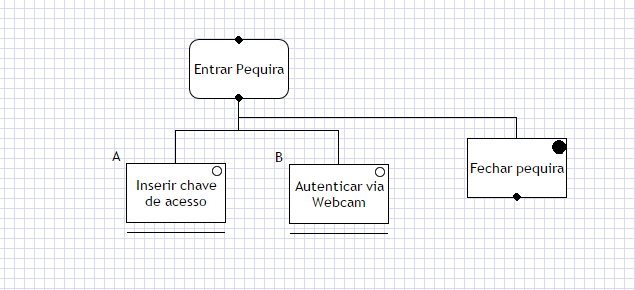
\includegraphics[scale=0.7]{MetaB.png}
\caption{Cenarios: 1 e 2 \quad Papel: Medico, Paciente}
\end{figure}

\subsection{Meta B - Usar Pequira}

\begin{figure}[h]
\centering
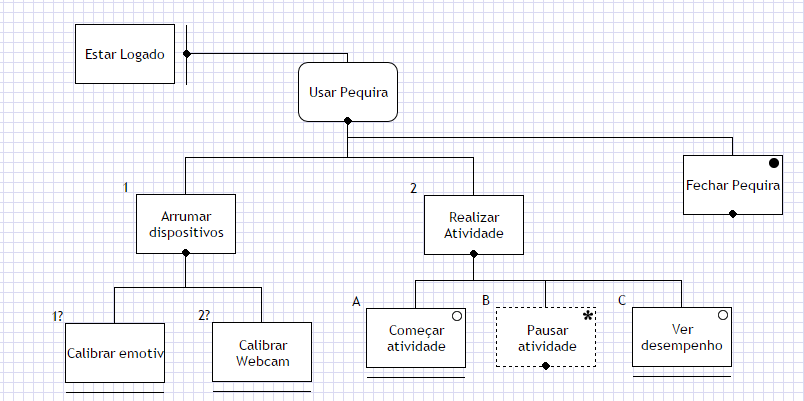
\includegraphics[scale=0.7]{MetaC.png}
\caption{Cenarios: 1,2,3 \quad Papel: Paciente}
\end{figure}
\paragraph{}
\begin{tabular}{lc}
1.1? & Usuário calibra os eletrodos do Emotiv. \\
1.2? & Usuário posiciona Webcam de forma que obtenha uma imagem frontal clara.
\end{tabular}
\newpage
\subsection{Meta C - Usar Pequira}

\begin{figure}[h]
\centering
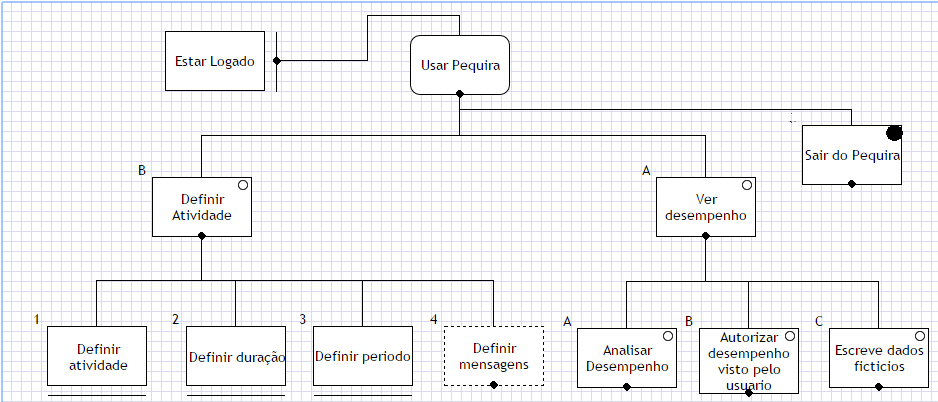
\includegraphics[scale=0.6]{MetaD.png}
\caption{Cenarios: 1,3 \quad Papel:Médico}
\end{figure}
\section{Considerações Finais}

\paragraph{} A modelagem ICH visa modelar as interações dos usuários com o sistema, bem como definir seus usuários e estabelecer qual a sua funcionalidade. Através deste trabalho é possível avaliar a dificuldade envolvida em atender um amplo público e observar os detalhes de interface que devem auxiliar o uso do sistema para o público almejado. Esta obriga os projetistas à se colocarem no lugar de seus usuários ao desenvolver cenários de uso, forçando uma reflexão que é utilizada em um futuro passo de prototipação.
%Com esse trabalho tivemos que construir a modelagem de IHC e com isso aprimoramos nosso conhecimento desta técnica. O trabalho também nos mostra a dificuldade de se tratar com questões de usabilidade e acessibilidade pois são muito detalhes que precisam ser pensados para que o sistema consiga tratar de forma eficiente cada um desses aspectos. Também temos a ambição de fazer com que os dados sejam gravados em nuvem para não termos mais a dependência do pendrive.



\begin{thebibliography}{99}                  
\bibitem{emotiv} EMOTIV \textbf{https://emotiv.com/}.
\end{thebibliography}     


\end{document}
